\documentclass[11pt, oneside]{article}   	% use "amsart" instead of "article" for AMSLaTeX format
\usepackage{geometry}                		% See geometry.pdf to learn the layout options. There are lots.
\geometry{letterpaper}                   		% ... or a4paper or a5paper or ... 
%\geometry{landscape}                		% Activate for for rotated page geometry
%\usepackage[parfill]{parskip}    		% Activate to begin paragraphs with an empty line rather than an indent
\usepackage{graphicx}				% Use pdf, png, jpg, or eps� with pdflatex; use eps in DVI mode
								% TeX will automatically convert eps --> pdf in pdflatex		
\usepackage{amssymb}
\usepackage{amsmath}

\title{Multiplication of matrices}
%\author{The Author}
\date{}							% Activate to display a given date or no date

\graphicspath{{/Users/telliott_admin/Dropbox/Tex/png/}}

\begin{document}

\maketitle
%\section{}
% \subsection*{R code}
% \begin{lstlisting}  \end{lstlisting}
% \begin{center} 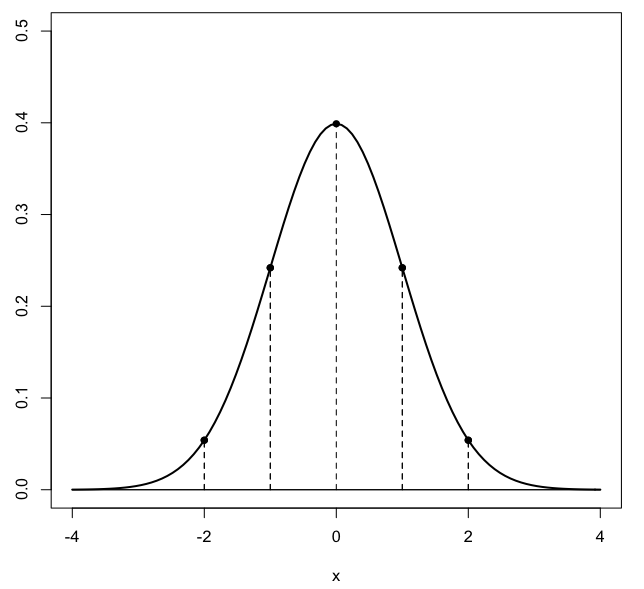
\includegraphics [scale=0.4] {gauss3.png} \end{center}
% \begin{bmatrix} a  &  b \\ c  &  d \end{bmatrix}
% \bigg |_

\large
\noindent
\subsection*{Standard picture}

Here is the figure from wikipedia.
\begin{center} 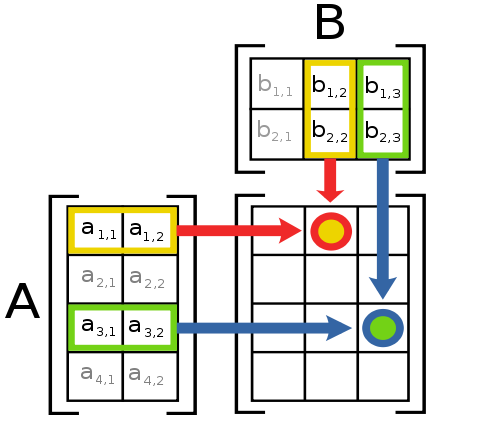
\includegraphics [scale=0.35] {mm1.png} \end{center}
First of all, note that for two matrices $A$ and $B$ to be multiplied together $A \times B$, the number of columns in $A$ must be equal to the number of rows in $B$. Here we have two columns in $A$ (it is a 4 x 2 matrix) and two rows in $B$ (a 2 x 3 matrix).
Let's call the product $P$ = $AB$.  Then, $P_{ij}$, the entry in row $i$, column $j$ of $P$, is obtained from the \emph{dot product} of row $i$ of $A$ $\cdot$ column $j$ of $B$.  In this case, there are two terms in each sum.  So
\[ P_{12} = a_{11} \ b_{12} + a_{12} \ b_{22} = row \ a_1 \cdot col \ b_2 \] 

If $A$ is an m x n matrix and $B$ is an n x p matrix, the result will be an m x p matrix, and each cofactor will be formed as the sum of n terms.

And in general, 
\[ P_{ij} = \sum_{k=1}^n a_{ik} \ b_{kj} \]

This is a little risky, but let's write out a $2 \times 2$ example where, as an experiment, I've labeled the subscripts going vertically in the second matrix
\[ M1 \times M2 = M1 \ M2 \]
\[
\begin{bmatrix}
a_1 & a_2 \\
b_1 & b_2 
\end{bmatrix}
\times
\begin{bmatrix}
c_1 & d_1 \\
c_2 & d_2 
\end{bmatrix}
= 
\begin{bmatrix}
a_1\ c_1 + a_2 \ c_2 & \ a_1\ d_1 + a_2 \ d_2 \\
b_1\ c_1 + b_2 \ c_2 & \ b_1\ d_1 + b_2 \ d_2
\end{bmatrix}
\]
In this arrangement, it's clear that the upper left entry is $\mathbf{a} \cdot \mathbf{c}$, where $\mathbf{a}$ is the first row of $M1$ and $\mathbf{c}$ is the first column of $M2$.

Here are two great pictures that I found on the web, which shows the dot product clearly.
\begin{center} 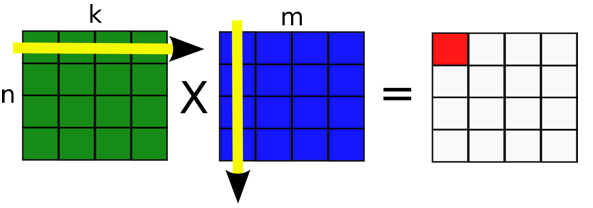
\includegraphics [scale=0.5] {mm2.png} \end{center}
\begin{center} 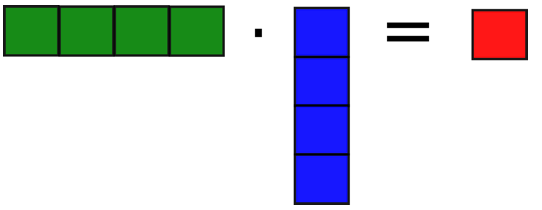
\includegraphics [scale=0.5] {mm3.png} \end{center}

It can be confusing keeping track of which row and column you are doing, or even whether it should be a row or a column.  That's why I really like the setup shown above in the wikipedia figure, where rather than write $A$ and $B$ on the same line, $A$ is written to the left of the space where $P$ will be filled in, and $B$ is shown above it.  Then it's clear which row and which column to choose when forming the sums.

\subsection*{Column picture}
The second way of looking at this same operation is introduced by thinking of the multiplication of a matrix $A$ times a vector $\mathbf{x}$ to give a second vector $A \times \mathbf{x} = \mathbf{b}$
\[
\begin{bmatrix}
a_{11} & a_{12} \\
a_{21} & a_{22} 
\end{bmatrix}
\times
\begin{bmatrix}
x_1 \\
x_2 
\end{bmatrix}
=
\begin{bmatrix}
b_1 \\
b_2 
\end{bmatrix}
\]
This is the same thing as
\[
x_1
\begin{bmatrix}
a_{11} \\
a_{21} 
\end{bmatrix}
+
x_2
\begin{bmatrix}
a_{12} \\
a_{22} 
\end{bmatrix}
\]
The result $\mathbf{b}$ is a \emph{combination} of the columns of $A$.  Here is a numerical example
\[
\begin{bmatrix}
1 & 2 \\
2 & 3 
\end{bmatrix}
\times
\begin{bmatrix}
1 \\
2 
\end{bmatrix}
=
\begin{bmatrix}
5 \\
8 
\end{bmatrix}
\]
This is the same thing as
\[
1
\begin{bmatrix}
1 \\
2
\end{bmatrix}
+
2
\begin{bmatrix}
2 \\
3 
\end{bmatrix}
=
\begin{bmatrix}
5 \\
8 
\end{bmatrix}
\]
\begin{center} 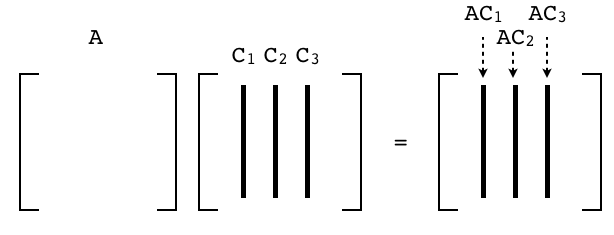
\includegraphics [scale=0.5] {mm4.png} \end{center}
This extends to a full matrix $B$ instead of the single vector $\mathbf{x}$.

Each of its columns $C_1$, $C_2$, etc. picks out a combination of the columns of $A$, and those combinations are what end up as the columns of the product.
\subsection*{Row picture}
In the same way, if we multiply (on the left) by a row vector---the transpose of a column vector---we see that the product is a combination of the rows of A.
$A \times \mathbf{x} = \mathbf{b}$
\[
\begin{bmatrix}
x_1 & x_2 
\end{bmatrix}
\times
\begin{bmatrix}
a_{11} & a_{12} \\
a_{21} & a_{22} 
\end{bmatrix}
=
\begin{bmatrix}
b_1 & b_2 
\end{bmatrix}
\]
This is the same thing as
\[
x_1
\begin{bmatrix}
a_{11} &  a_{21} 
\end{bmatrix}
+
x_2
\begin{bmatrix}
a_{12} & a_{22} 
\end{bmatrix}
=
\begin{bmatrix}
b_1 & b_2 
\end{bmatrix}
\]
Here is a numerical example
\[
\begin{bmatrix}
1 & 2 
\end{bmatrix}
\times
\begin{bmatrix}
1 & 2 \\
2 & 3 
\end{bmatrix}
=
\begin{bmatrix}
5 & 8 
\end{bmatrix}
\]
This is the same thing as
\[
1
\begin{bmatrix}
1 &  2 
\end{bmatrix}
+
2
\begin{bmatrix}
2 & 3 
\end{bmatrix}
=
\begin{bmatrix}
5 & 8 
\end{bmatrix}
\]
\begin{center} 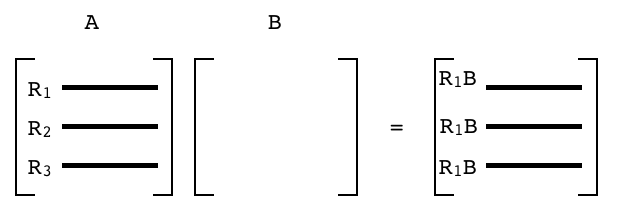
\includegraphics [scale=0.5] {mm5.png} \end{center}

\subsection*{One row and one column}
\[
\begin{bmatrix}
a_1 & a_2 & a_3 
\end{bmatrix}
\begin{bmatrix}
b_1 \\ 
b_2 \\ 
b_3 
\end{bmatrix}
=
\begin{bmatrix}
a_1\ b_1 & a_1\ b_2 & a_1\ b_3 \\
a_2\ b_1 & a_2\ b_2 & a_2\ b_3 \\
a_3\ b_1 & a_3\ b_2 & a_3\ b_3
\end{bmatrix}
\]
For each row of $A$ we find the correct column of $B$ and do this multiplication, generating a whole series of matrices of full size.  Then we add together all the matrices.
\subsection*{Blocks}
The fifth and last view of matrix multiplication involves thinking about regions derived from the original matrix but containing a number of elements.
\begin{center} 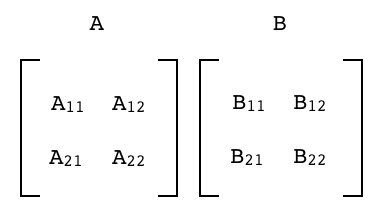
\includegraphics [scale=0.6] {mm6.png} \end{center}

The upper-left hand corner (2 x 2) would be formed by $A_11 \times B_11 + A_21 \times B_12$.

For example, with these two 4 x 4 matrices
\[
\begin{bmatrix}
a & b & c & d \\
e & f & g & h \\
i & j & k & l \\
m & n & o & p \\
\end{bmatrix}
\times
\begin{bmatrix}
A & B & C & D \\
E & F & G & H \\
I & J & K & L \\
M & N & O & P \\
\end{bmatrix}
=
\]
The entry in row 1, column 1 is computed in the standard "dot product" way as $aA + bE + cI + dM$, but if you broke it up into blocks the upper left-hand corner (a 2 x 2 matrix) would be computed as follows
\[
\begin{bmatrix}
a & b \\
e & f \\
\end{bmatrix}
\times
\begin{bmatrix}
A & B  \\
E & F \\
\end{bmatrix}
+
\begin{bmatrix}
c & d \\
g & h \\
\end{bmatrix}
\times
\begin{bmatrix}
I & J  \\
M & N \\
\end{bmatrix}
\]
\[ =
\begin{bmatrix}
aA + bE & aB + bF  \\
eA + fE & eB + fF  \\
\end{bmatrix}
+
\begin{bmatrix}
cI + dM & cJ + dN  \\
gI + hM & gJ + hN  \\
\end{bmatrix}
\]
I won't fill in the whole thing, but you can see that the entry in row 1, column 1 is indeed $aA + bE + cI + dM $.

\end{document}  